\documentclass[english]{beamer}
\mode<presentation>

%\usepackage[slovak]{babel}
\usepackage[utf8]{inputenc}
\usepackage{physics}
\usepackage{tikz, pgfplots}
%\DeclareMathSizes{12pt}{10pt}{10pt}{10pt}

\usepackage{multimedia}
\RequirePackage{environ}

\usepackage{changepage}
\makeatletter
\newenvironment{forcecenter}%
    {\@parboxrestore%
     \begin{adjustwidth}{}{\leftmargin}%
    }{\end{adjustwidth}
     }
\makeatother

%\graphicspath{images}

%Use Okular!

\newcommand\Wider[2][3em]{
\makebox{\linewidth][c]{
	\begin{minipage}{\dimexpr\textwidth+#1\relax}
	\raggedright#2
	\end{minipage}	
	}
}
}

\NewEnviron{sea}{
	\fontsize{9}{12}
    \begin{eqnarray*}
   % \fontsize{12pt}{10pt}\selectfont
    \BODY
    \end{eqnarray*}
    \normalsize
}

\begin{document}

  \title{Research Experience: A Study of Symmetry Elevation in InGaAs Quantum Dots}
  \author[Michal Horanský]{Michal Horanský\\\hfill\\Imperial College London}
  %\date{14. apríl 2019}
  %\maketitle
  \date{January 10, 2024}
  \begin{frame}
    \titlepage
  \end{frame}
    %\begin{center}
    %\includegraphics<1->[scale=0.5]{images/multipendulum_scheme.png}
    %\end{center}
  
  
  \begin{frame}
  	\frametitle{Introduction}
  	\framesubtitle{An outline of the problem}
  	\begin{itemize}
  		\item Master's project (MSci) under Professor Dimitri Vvedensky at Imperial College London
  		\item Collaboration with Professor Stefan Schulz (UCC) and Professor Emanuele Pelucchi (Tyndall Institute)
  		\item Problem specifics:
  		\begin{itemize}
  		\item Quantum dots with high spatial symmetry: photoluminiscence
  		\item Fine-structure splitting of excitonic energy levels
  		\item Resolvable peaks within major features of the photoluminiscence spectrum
  		\item Symmetry elevation
  		\end{itemize}
  	\end{itemize}
  \end{frame}
  
  \begin{frame}
  	\frametitle{Introduction}
  	\framesubtitle{The quantum dot in question}
  	
  	\begin{figure}
	\centering
    		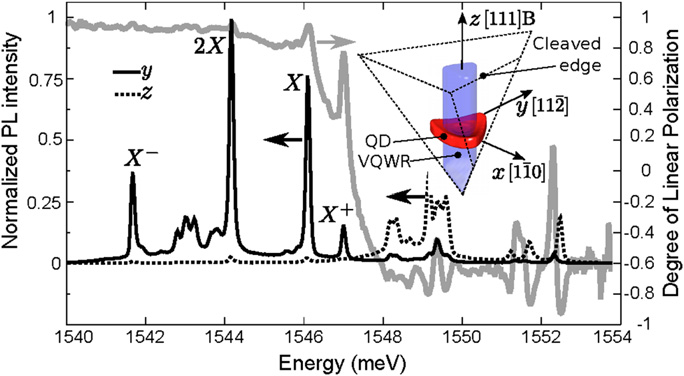
\includegraphics[width=0.9\textwidth]{images/QD_schematic}
    		\caption{Gross spectrum of a $C_{3v}$ InGaAs QD. Image credit: Karlsson, K. F. et al (2015), Spectral signatures of high-symmetry quantum dots and effects of symmetry breaking. New Journal of Physics, 17 103017}
    		\label{fig:qd}
	\end{figure}
\end{frame}

	\begin{frame}
		\frametitle{Introduction}
		\framesubtitle{Exciton energy levels and transitions}
		\begin{figure}
	\centering
    		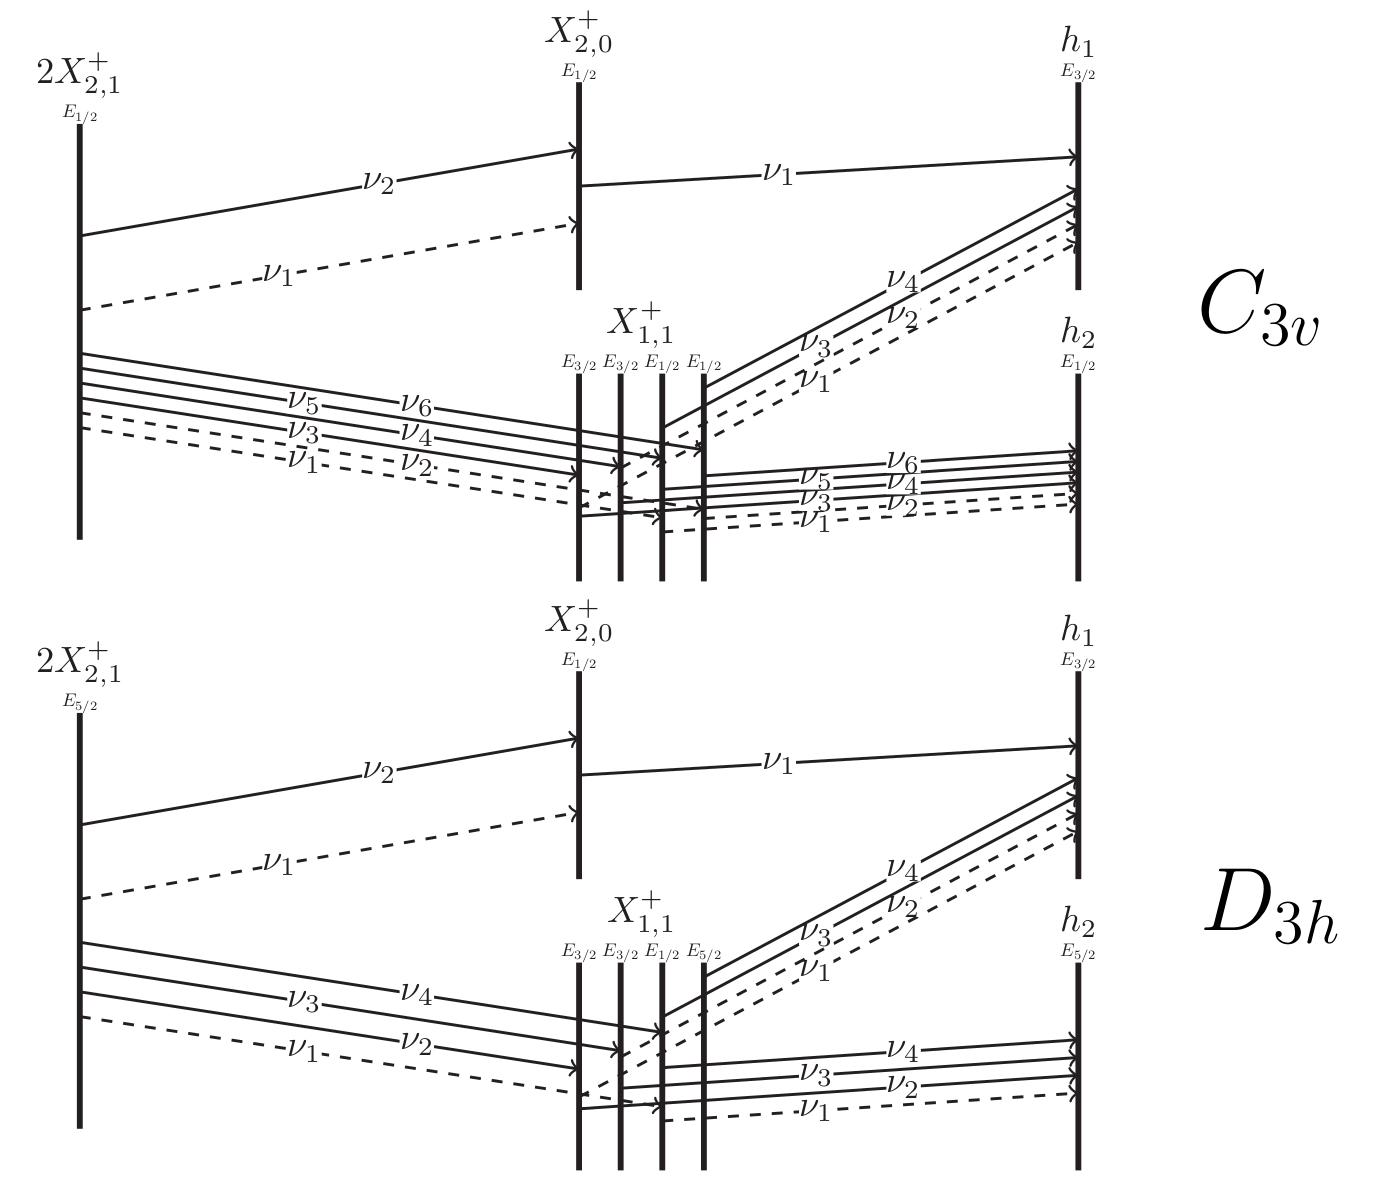
\includegraphics[width=0.85\textwidth]{images/2X21_scheme}
    		\label{fig:qd}
	\end{figure}
		
	
	
	\end{frame}
  
  \begin{frame}
  	\frametitle{Approach}
  	%\framesubtitle{MSci third-year group project at ICL}
  	\begin{itemize}
  		\item Tight-binding model with fine-structure: angular momentum paradigm
  		\item Group theory: $j$-coupling, energy level splitting, selection rules
  		\item $k\cdot p$ theory: L-K in the vicininty of $\Gamma$
  	\end{itemize}
  \end{frame}
  
  \begin{frame}
  	\frametitle{My contribution and results}
  	\begin{itemize}
  		\item AReTDoG: Algorithms for Representation Theory of Double Groups
		\begin{itemize}		  		
  			\item Non-trivial construction of time-reversal symmetry
  			\item $SO(3)\to SU(2)$ injection
  			\item Fermionic characters as results of symmetry breaking of $SU(2)$ Wigner-like irreps
		\end{itemize}
  		\item Identification of band-mixing effects and Bloch-periodic potential as two candidates for symmetry-elevation causes
  		\item A novel treatment of inversion symmetry $\hat{P}$ within angular-momentum coupling group-theoretical formalism (parity as a required quantum number)
  		
  		
  	\end{itemize}
  \end{frame}
  
  \begin{frame}
  	\frametitle{Outlook on the future}
  	
  	\begin{itemize}
  		\item To do: evaulate the magnitudes of band-mixing effects and inner-lattice effects to check whether they can explain symmetry elevation
  		\item Extending the project for a summer research placement (UROP) to build a concise picture of the entire system, beyond the formalism of Karlsson et al.
  		\item Cross-reference with experimental and computational results
  	\end{itemize}
  
  
  \end{frame}
  

\end{document}